% Options for packages loaded elsewhere
\PassOptionsToPackage{unicode}{hyperref}
\PassOptionsToPackage{hyphens}{url}
\PassOptionsToPackage{dvipsnames,svgnames,x11names}{xcolor}
%
\documentclass[
  letterpaper,
  DIV=11,
  numbers=noendperiod]{scrartcl}

\usepackage{amsmath,amssymb}
\usepackage{iftex}
\ifPDFTeX
  \usepackage[T1]{fontenc}
  \usepackage[utf8]{inputenc}
  \usepackage{textcomp} % provide euro and other symbols
\else % if luatex or xetex
  \usepackage{unicode-math}
  \defaultfontfeatures{Scale=MatchLowercase}
  \defaultfontfeatures[\rmfamily]{Ligatures=TeX,Scale=1}
\fi
\usepackage{lmodern}
\ifPDFTeX\else  
    % xetex/luatex font selection
\fi
% Use upquote if available, for straight quotes in verbatim environments
\IfFileExists{upquote.sty}{\usepackage{upquote}}{}
\IfFileExists{microtype.sty}{% use microtype if available
  \usepackage[]{microtype}
  \UseMicrotypeSet[protrusion]{basicmath} % disable protrusion for tt fonts
}{}
\makeatletter
\@ifundefined{KOMAClassName}{% if non-KOMA class
  \IfFileExists{parskip.sty}{%
    \usepackage{parskip}
  }{% else
    \setlength{\parindent}{0pt}
    \setlength{\parskip}{6pt plus 2pt minus 1pt}}
}{% if KOMA class
  \KOMAoptions{parskip=half}}
\makeatother
\usepackage{xcolor}
\ifLuaTeX
  \usepackage{luacolor}
  \usepackage[soul]{lua-ul}
\else
  \usepackage{soul}
  
\fi
\setlength{\emergencystretch}{3em} % prevent overfull lines
\setcounter{secnumdepth}{-\maxdimen} % remove section numbering
% Make \paragraph and \subparagraph free-standing
\makeatletter
\ifx\paragraph\undefined\else
  \let\oldparagraph\paragraph
  \renewcommand{\paragraph}{
    \@ifstar
      \xxxParagraphStar
      \xxxParagraphNoStar
  }
  \newcommand{\xxxParagraphStar}[1]{\oldparagraph*{#1}\mbox{}}
  \newcommand{\xxxParagraphNoStar}[1]{\oldparagraph{#1}\mbox{}}
\fi
\ifx\subparagraph\undefined\else
  \let\oldsubparagraph\subparagraph
  \renewcommand{\subparagraph}{
    \@ifstar
      \xxxSubParagraphStar
      \xxxSubParagraphNoStar
  }
  \newcommand{\xxxSubParagraphStar}[1]{\oldsubparagraph*{#1}\mbox{}}
  \newcommand{\xxxSubParagraphNoStar}[1]{\oldsubparagraph{#1}\mbox{}}
\fi
\makeatother

\usepackage{color}
\usepackage{fancyvrb}
\newcommand{\VerbBar}{|}
\newcommand{\VERB}{\Verb[commandchars=\\\{\}]}
\DefineVerbatimEnvironment{Highlighting}{Verbatim}{commandchars=\\\{\}}
% Add ',fontsize=\small' for more characters per line
\usepackage{framed}
\definecolor{shadecolor}{RGB}{241,243,245}
\newenvironment{Shaded}{\begin{snugshade}}{\end{snugshade}}
\newcommand{\AlertTok}[1]{\textcolor[rgb]{0.68,0.00,0.00}{#1}}
\newcommand{\AnnotationTok}[1]{\textcolor[rgb]{0.37,0.37,0.37}{#1}}
\newcommand{\AttributeTok}[1]{\textcolor[rgb]{0.40,0.45,0.13}{#1}}
\newcommand{\BaseNTok}[1]{\textcolor[rgb]{0.68,0.00,0.00}{#1}}
\newcommand{\BuiltInTok}[1]{\textcolor[rgb]{0.00,0.23,0.31}{#1}}
\newcommand{\CharTok}[1]{\textcolor[rgb]{0.13,0.47,0.30}{#1}}
\newcommand{\CommentTok}[1]{\textcolor[rgb]{0.37,0.37,0.37}{#1}}
\newcommand{\CommentVarTok}[1]{\textcolor[rgb]{0.37,0.37,0.37}{\textit{#1}}}
\newcommand{\ConstantTok}[1]{\textcolor[rgb]{0.56,0.35,0.01}{#1}}
\newcommand{\ControlFlowTok}[1]{\textcolor[rgb]{0.00,0.23,0.31}{\textbf{#1}}}
\newcommand{\DataTypeTok}[1]{\textcolor[rgb]{0.68,0.00,0.00}{#1}}
\newcommand{\DecValTok}[1]{\textcolor[rgb]{0.68,0.00,0.00}{#1}}
\newcommand{\DocumentationTok}[1]{\textcolor[rgb]{0.37,0.37,0.37}{\textit{#1}}}
\newcommand{\ErrorTok}[1]{\textcolor[rgb]{0.68,0.00,0.00}{#1}}
\newcommand{\ExtensionTok}[1]{\textcolor[rgb]{0.00,0.23,0.31}{#1}}
\newcommand{\FloatTok}[1]{\textcolor[rgb]{0.68,0.00,0.00}{#1}}
\newcommand{\FunctionTok}[1]{\textcolor[rgb]{0.28,0.35,0.67}{#1}}
\newcommand{\ImportTok}[1]{\textcolor[rgb]{0.00,0.46,0.62}{#1}}
\newcommand{\InformationTok}[1]{\textcolor[rgb]{0.37,0.37,0.37}{#1}}
\newcommand{\KeywordTok}[1]{\textcolor[rgb]{0.00,0.23,0.31}{\textbf{#1}}}
\newcommand{\NormalTok}[1]{\textcolor[rgb]{0.00,0.23,0.31}{#1}}
\newcommand{\OperatorTok}[1]{\textcolor[rgb]{0.37,0.37,0.37}{#1}}
\newcommand{\OtherTok}[1]{\textcolor[rgb]{0.00,0.23,0.31}{#1}}
\newcommand{\PreprocessorTok}[1]{\textcolor[rgb]{0.68,0.00,0.00}{#1}}
\newcommand{\RegionMarkerTok}[1]{\textcolor[rgb]{0.00,0.23,0.31}{#1}}
\newcommand{\SpecialCharTok}[1]{\textcolor[rgb]{0.37,0.37,0.37}{#1}}
\newcommand{\SpecialStringTok}[1]{\textcolor[rgb]{0.13,0.47,0.30}{#1}}
\newcommand{\StringTok}[1]{\textcolor[rgb]{0.13,0.47,0.30}{#1}}
\newcommand{\VariableTok}[1]{\textcolor[rgb]{0.07,0.07,0.07}{#1}}
\newcommand{\VerbatimStringTok}[1]{\textcolor[rgb]{0.13,0.47,0.30}{#1}}
\newcommand{\WarningTok}[1]{\textcolor[rgb]{0.37,0.37,0.37}{\textit{#1}}}

\providecommand{\tightlist}{%
  \setlength{\itemsep}{0pt}\setlength{\parskip}{0pt}}\usepackage{longtable,booktabs,array}
\usepackage{calc} % for calculating minipage widths
% Correct order of tables after \paragraph or \subparagraph
\usepackage{etoolbox}
\makeatletter
\patchcmd\longtable{\par}{\if@noskipsec\mbox{}\fi\par}{}{}
\makeatother
% Allow footnotes in longtable head/foot
\IfFileExists{footnotehyper.sty}{\usepackage{footnotehyper}}{\usepackage{footnote}}
\makesavenoteenv{longtable}
\usepackage{graphicx}
\makeatletter
\def\maxwidth{\ifdim\Gin@nat@width>\linewidth\linewidth\else\Gin@nat@width\fi}
\def\maxheight{\ifdim\Gin@nat@height>\textheight\textheight\else\Gin@nat@height\fi}
\makeatother
% Scale images if necessary, so that they will not overflow the page
% margins by default, and it is still possible to overwrite the defaults
% using explicit options in \includegraphics[width, height, ...]{}
\setkeys{Gin}{width=\maxwidth,height=\maxheight,keepaspectratio}
% Set default figure placement to htbp
\makeatletter
\def\fps@figure{htbp}
\makeatother

\KOMAoption{captions}{tableheading}
\makeatletter
\@ifpackageloaded{caption}{}{\usepackage{caption}}
\AtBeginDocument{%
\ifdefined\contentsname
  \renewcommand*\contentsname{Table of contents}
\else
  \newcommand\contentsname{Table of contents}
\fi
\ifdefined\listfigurename
  \renewcommand*\listfigurename{List of Figures}
\else
  \newcommand\listfigurename{List of Figures}
\fi
\ifdefined\listtablename
  \renewcommand*\listtablename{List of Tables}
\else
  \newcommand\listtablename{List of Tables}
\fi
\ifdefined\figurename
  \renewcommand*\figurename{Figure}
\else
  \newcommand\figurename{Figure}
\fi
\ifdefined\tablename
  \renewcommand*\tablename{Table}
\else
  \newcommand\tablename{Table}
\fi
}
\@ifpackageloaded{float}{}{\usepackage{float}}
\floatstyle{ruled}
\@ifundefined{c@chapter}{\newfloat{codelisting}{h}{lop}}{\newfloat{codelisting}{h}{lop}[chapter]}
\floatname{codelisting}{Listing}
\newcommand*\listoflistings{\listof{codelisting}{List of Listings}}
\makeatother
\makeatletter
\makeatother
\makeatletter
\@ifpackageloaded{caption}{}{\usepackage{caption}}
\@ifpackageloaded{subcaption}{}{\usepackage{subcaption}}
\makeatother

\ifLuaTeX
  \usepackage{selnolig}  % disable illegal ligatures
\fi
\usepackage{bookmark}

\IfFileExists{xurl.sty}{\usepackage{xurl}}{} % add URL line breaks if available
\urlstyle{same} % disable monospaced font for URLs
\hypersetup{
  pdftitle={MATH 3190 Homework 1},
  colorlinks=true,
  linkcolor={blue},
  filecolor={Maroon},
  citecolor={Blue},
  urlcolor={blue},
  pdfcreator={LaTeX via pandoc}}


\title{\textbf{MATH 3190 Homework 1}}
\usepackage{etoolbox}
\makeatletter
\providecommand{\subtitle}[1]{% add subtitle to \maketitle
  \apptocmd{\@title}{\par {\large #1 \par}}{}{}
}
\makeatother
\subtitle{Due January 29, 2026\\
Focus: Notes 1-3\\
Total Points: 90 + 10 (Self-Critique Comment and Uploading to GitHub) =
100}
\author{}
\date{}

\begin{document}
\maketitle


Note that your homework should be completed in Quarto. You can just add
your answers and code to this document in the appropriate part. The file
should be rendered as an html document or pdf document (html is quicker
to render and you will need an installation of LaTeX to render as a
pdf). You will ``turn in'' this homework by uploading the files, the
.qmd and output file, to your GitHub \texttt{Math\_3190\_Assignment}
repository in the \texttt{Homework/Homework\_1} directory. Make sure all
supporting files (if there are any) are in this directory as well. You
should use \texttt{git} and \texttt{Unix} commands in a terminal for
this (i.e.~don't manually upload files to GitHub). In addition, you will
submit just your html or pdf file on Canvas to unlock the solutions.

Don't forget to also put a \ul{self-critique comment} on Canvas
indicating what you did correctly and incorrectly and include any
questions you may have about the assignment after submitting the
assignment and thoroughly looking through the solutions.

\section{Problem 1 (18 points)}\label{problem-1-18-points}

In \ul{two different code chunks}, write two functions called
\texttt{gghist} and \texttt{ggbox}. The first code chunk is already
given below, but you'll need to add the second one. The \texttt{gghist}
function should create a ggplot histogram of a variable that is given as
a vector. The \texttt{ggbox} function should create a ggplot box plot
when a single numeric vector is given or it should create side-by-side
box plots if one numeric and one categorical variables are given. You
can check if a vector is numeric with the \texttt{is.numeric()}
function. Allow the user to indicate whether it should be horizontal or
vertical box plots. Make sure you set \texttt{echo} and \texttt{eval}
both to \texttt{true} for these code chunks. Also make sure to label the
code chunks.

\begin{Shaded}
\begin{Highlighting}[]
\CommentTok{\# Put gghist function here.}
\NormalTok{gghist }\OtherTok{=} \ControlFlowTok{function}\NormalTok{(x) \{}
  \FunctionTok{hist}\NormalTok{(x)}
\NormalTok{  return}
\NormalTok{\}}

\FunctionTok{gghist}\NormalTok{(}\FunctionTok{c}\NormalTok{(}\DecValTok{2}\NormalTok{,}\DecValTok{4}\NormalTok{,}\DecValTok{6}\NormalTok{,}\DecValTok{7}\NormalTok{,}\DecValTok{10}\NormalTok{,}\DecValTok{16}\NormalTok{))}
\end{Highlighting}
\end{Shaded}

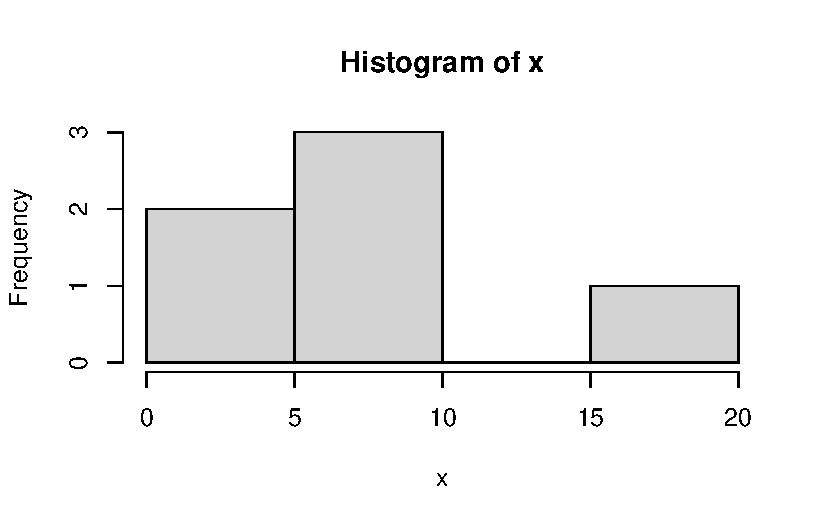
\includegraphics{Homework-1_files/figure-pdf/gghist-1.pdf}

\begin{verbatim}
.Primitive("return")
\end{verbatim}

\begin{Shaded}
\begin{Highlighting}[]
\NormalTok{ggbox }\OtherTok{\textless{}{-}} \ControlFlowTok{function}\NormalTok{(df, x, y) \{}
  \FunctionTok{ggplot}\NormalTok{(df, }\FunctionTok{aes}\NormalTok{(}\AttributeTok{x =}\NormalTok{ \{\{x\}\}, }\AttributeTok{y =}\NormalTok{ \{\{y\}\})) }\SpecialCharTok{+}
    \FunctionTok{geom\_boxplot}\NormalTok{()}
\NormalTok{\}}
\end{Highlighting}
\end{Shaded}

\section{Problem 2 (57 points)}\label{problem-2-57-points}

\subsubsection{Part a (6 points)}\label{part-a-6-points}

Learn about the built-in \texttt{read.fwf()} \textbf{R} function for use
in downloading data from a URL into \textbf{R}. The \texttt{widths} and
\texttt{strip.white} options will be especially useful here. Use this
function to download the scores for all college basketball games for the
2024-2025 season \url{http://kenpom.com/cbbga26.txt} and then convert it
to a tibble (load the \texttt{tidyverse} package first). The second team
listed per line is the home team. It is not clear what the numbers,
letters, or city names indicate after the second listed score. Notice
that this is a ``live'' file that gets updated every day! So, your
tibble size may change if you work on this assignment over the course of
several days. That's fine. Give the code you used to download these data
in a labeled code chunk.

\begin{Shaded}
\begin{Highlighting}[]
\FunctionTok{library}\NormalTok{(tidyverse)}
\end{Highlighting}
\end{Shaded}

\begin{verbatim}
Warning: package 'ggplot2' was built under R version 4.4.3
\end{verbatim}

\begin{verbatim}
Warning: package 'tibble' was built under R version 4.4.3
\end{verbatim}

\begin{verbatim}
Warning: package 'purrr' was built under R version 4.4.3
\end{verbatim}

\begin{verbatim}
Warning: package 'stringr' was built under R version 4.4.3
\end{verbatim}

\begin{verbatim}
-- Attaching core tidyverse packages ------------------------ tidyverse 2.0.0 --
v dplyr     1.1.4     v readr     2.1.5
v forcats   1.0.0     v stringr   1.5.2
v ggplot2   4.0.0     v tibble    3.3.0
v lubridate 1.9.4     v tidyr     1.3.1
v purrr     1.1.0     
-- Conflicts ------------------------------------------ tidyverse_conflicts() --
x dplyr::filter() masks stats::filter()
x dplyr::lag()    masks stats::lag()
i Use the conflicted package (<http://conflicted.r-lib.org/>) to force all conflicts to become errors
\end{verbatim}

\begin{Shaded}
\begin{Highlighting}[]
\NormalTok{cbbga }\OtherTok{=} \FunctionTok{read.fwf}\NormalTok{(}\StringTok{\textquotesingle{}http://kenpom.com/cbbga26.txt\textquotesingle{}}\NormalTok{, }\AttributeTok{widths =} \FunctionTok{c}\NormalTok{(}\DecValTok{10}\NormalTok{, }\DecValTok{24}\NormalTok{, }\DecValTok{4}\NormalTok{, }\DecValTok{23}\NormalTok{, }\DecValTok{5}\NormalTok{, }\DecValTok{10}\NormalTok{), }\AttributeTok{strip.white=}\ConstantTok{TRUE}\NormalTok{)}
\FunctionTok{as.tibble}\NormalTok{(cbbga)}
\end{Highlighting}
\end{Shaded}

\begin{verbatim}
Warning: `as.tibble()` was deprecated in tibble 2.0.0.
i Please use `as_tibble()` instead.
i The signature and semantics have changed, see `?as_tibble`.
\end{verbatim}

\begin{verbatim}
# A tibble: 4,089 x 6
   V1         V2                 V3 V4                V5    V6       
   <chr>      <chr>           <int> <chr>             <chr> <chr>    
 1 11/03/2025 McMurry            55 Abilene Christian 92    ""       
 2 11/03/2025 James Madison      71 Akron             85    ""       
 3 11/03/2025 North Dakota       62 Alabama           91    ""       
 4 11/03/2025 Blue Mountain      60 Alabama A&M       80    ""       
 5 11/03/2025 Florida            87 Arizona           93 N  "Las Veg"
 6 11/03/2025 Southern           77 Arkansas          109   ""       
 7 11/03/2025 SUNY Maritime      49 Army              73    ""       
 8 11/03/2025 Bethune Cookman    90 Auburn            95 1  ""       
 9 11/03/2025 Bryan              47 Austin Peay       128   ""       
10 11/03/2025 Louisiana          64 Ball St.          75    ""       
# i 4,079 more rows
\end{verbatim}

Now lets practice using our tidy data/tidyverse tools! Using your
\texttt{cbbga} tibble, try doing the following. In each part, save the
object as a new tibble (like \texttt{cbbga2}, \texttt{cbbga3}, etc) and
in each subsequent part, use the tibble you created in the previous
part.

\subsubsection{Part b (2 points)}\label{part-b-2-points}

Use \texttt{rename()} to rename all of your variables to names that make
sense. Then print the first six rows of the new tibble using the
\texttt{head()} function.

\begin{Shaded}
\begin{Highlighting}[]
\NormalTok{cbbga2 }\OtherTok{=} \FunctionTok{rename}\NormalTok{(cbbga, }\AttributeTok{date =}\NormalTok{ V1, }\AttributeTok{visitor =}\NormalTok{ V2, }\AttributeTok{visitor\_score =}\NormalTok{ V3, }\AttributeTok{home =}\NormalTok{ V4, }\AttributeTok{home\_score =}\NormalTok{ V5)}
\FunctionTok{head}\NormalTok{(cbbga2)}
\end{Highlighting}
\end{Shaded}

\begin{verbatim}
        date       visitor visitor_score              home home_score      V6
1 11/03/2025       McMurry            55 Abilene Christian         92        
2 11/03/2025 James Madison            71             Akron         85        
3 11/03/2025  North Dakota            62           Alabama         91        
4 11/03/2025 Blue Mountain            60       Alabama A&M         80        
5 11/03/2025       Florida            87           Arizona       93 N Las Veg
6 11/03/2025      Southern            77          Arkansas        109        
\end{verbatim}

\subsubsection{Part c (2 points)}\label{part-c-2-points}

Use \texttt{mutate()} to create a new column that gives the score
differences (home team score minus away team score). Then print the
first six rows of the new tibble using the \texttt{head()} function.

\begin{Shaded}
\begin{Highlighting}[]
\NormalTok{cbbga3 }\OtherTok{=}\NormalTok{ cbbga2 }\SpecialCharTok{|\textgreater{}}
  \FunctionTok{mutate}\NormalTok{(}\AttributeTok{home\_score =} \FunctionTok{gsub}\NormalTok{(}\StringTok{"[\^{}0{-}9.]"}\NormalTok{, }\StringTok{""}\NormalTok{, cbbga2}\SpecialCharTok{$}\NormalTok{home\_score)) }\SpecialCharTok{|\textgreater{}}
  \FunctionTok{mutate}\NormalTok{(}\AttributeTok{score\_difference =} \FunctionTok{as.numeric}\NormalTok{(home\_score) }\SpecialCharTok{{-}} \FunctionTok{as.numeric}\NormalTok{(visitor\_score))}

\FunctionTok{head}\NormalTok{(cbbga3)}
\end{Highlighting}
\end{Shaded}

\begin{verbatim}
        date       visitor visitor_score              home home_score      V6
1 11/03/2025       McMurry            55 Abilene Christian         92        
2 11/03/2025 James Madison            71             Akron         85        
3 11/03/2025  North Dakota            62           Alabama         91        
4 11/03/2025 Blue Mountain            60       Alabama A&M         80        
5 11/03/2025       Florida            87           Arizona         93 Las Veg
6 11/03/2025      Southern            77          Arkansas        109        
  score_difference
1               37
2               14
3               29
4               20
5                6
6               32
\end{verbatim}

\subsubsection{Part d (2 points)}\label{part-d-2-points}

Use \texttt{arrange()} to sort the data set by the home team
alphabetically. Then print the first six rows of t

\begin{Shaded}
\begin{Highlighting}[]
\NormalTok{cbbga4 }\OtherTok{=} \FunctionTok{arrange}\NormalTok{(cbbga3, home)}

\FunctionTok{head}\NormalTok{(cbbga)}
\end{Highlighting}
\end{Shaded}

\begin{verbatim}
          V1            V2 V3                V4   V5      V6
1 11/03/2025       McMurry 55 Abilene Christian   92        
2 11/03/2025 James Madison 71             Akron   85        
3 11/03/2025  North Dakota 62           Alabama   91        
4 11/03/2025 Blue Mountain 60       Alabama A&M   80        
5 11/03/2025       Florida 87           Arizona 93 N Las Veg
6 11/03/2025      Southern 77          Arkansas  109        
\end{verbatim}

he new tibble using the \texttt{head()} function.

\subsubsection{Part e (2 points)}\label{part-e-2-points}

Use \texttt{select()} to remove the extra variable(s) that had that
irrelevant information at the end of each line. Note: you can select
every variable except one by using \texttt{!}. Then print the first six
rows of the new tibble using the \texttt{head()} function.

\begin{Shaded}
\begin{Highlighting}[]
\NormalTok{cbbga5 }\OtherTok{=} \FunctionTok{select}\NormalTok{(cbbga4, }\SpecialCharTok{!}\NormalTok{V6)}
\end{Highlighting}
\end{Shaded}

\subsubsection{Part f (3 points)}\label{part-f-3-points}

Put parts a-e all together in one piping expression (with 5 pipes) and
save this as a new object in \textbf{R}.

\begin{Shaded}
\begin{Highlighting}[]
\NormalTok{object }\OtherTok{=}\NormalTok{ cbbga }\SpecialCharTok{|\textgreater{}}
  \FunctionTok{rename}\NormalTok{(}\AttributeTok{date =}\NormalTok{ V1, }\AttributeTok{visitor =}\NormalTok{ V2, }\AttributeTok{visitor\_score =}\NormalTok{ V3, }\AttributeTok{home =}\NormalTok{ V4, }\AttributeTok{home\_score =}\NormalTok{ V5) }\SpecialCharTok{|\textgreater{}}
  \FunctionTok{mutate}\NormalTok{(}\AttributeTok{home\_score =} \FunctionTok{gsub}\NormalTok{(}\StringTok{"[\^{}0{-}9.]"}\NormalTok{, }\StringTok{""}\NormalTok{, cbbga2}\SpecialCharTok{$}\NormalTok{home\_score)) }\SpecialCharTok{|\textgreater{}}
  \FunctionTok{mutate}\NormalTok{(}\AttributeTok{score\_difference =} \FunctionTok{as.numeric}\NormalTok{(home\_score) }\SpecialCharTok{{-}} \FunctionTok{as.numeric}\NormalTok{(visitor\_score))}\SpecialCharTok{|\textgreater{}}
  \FunctionTok{arrange}\NormalTok{(home)}\SpecialCharTok{|\textgreater{}}
  \FunctionTok{select}\NormalTok{(}\SpecialCharTok{!}\NormalTok{V6)}

\FunctionTok{saveRDS}\NormalTok{(object, }\AttributeTok{file =} \StringTok{\textquotesingle{}cbbga.rds\textquotesingle{}}\NormalTok{)}
\end{Highlighting}
\end{Shaded}

\subsubsection{Part g (3 points)}\label{part-g-3-points}

Use \texttt{filter()} to reduce the data down to only games played in
2025 (you could use the \texttt{lubridate} package for this, since it
specializes in dealing with dates, but some base \textbf{R} packages
will also work). Save this in a new tibble. \textbf{We will use this
tibble with only the 2025 years from here on out}.

\begin{Shaded}
\begin{Highlighting}[]
\NormalTok{cbbga5}\SpecialCharTok{$}\NormalTok{date }\OtherTok{=} \FunctionTok{as.Date}\NormalTok{(cbbga5}\SpecialCharTok{$}\NormalTok{date, }\AttributeTok{format =} \StringTok{"\%m/\%d/\%Y"}\NormalTok{)}
\NormalTok{cbbga6 }\OtherTok{=}\NormalTok{ cbbga5 }\SpecialCharTok{|\textgreater{}}
  \FunctionTok{filter}\NormalTok{(date }\SpecialCharTok{\textgreater{}}\StringTok{"2024{-}12{-}31"}\NormalTok{) }\SpecialCharTok{|\textgreater{}}
  \FunctionTok{filter}\NormalTok{(date}\SpecialCharTok{\textless{}}\StringTok{"2026{-}01{-}01"}\NormalTok{)}
\end{Highlighting}
\end{Shaded}

\subsubsection{Part h (4 points)}\label{part-h-4-points}

Write a function that will filter the tibble to only games played by a
given team. Demonstrate your function by displaying games played by SUU
in 2025.

\begin{Shaded}
\begin{Highlighting}[]
\NormalTok{team\_filter }\OtherTok{\textless{}{-}} \ControlFlowTok{function}\NormalTok{(x) \{}
\NormalTok{  df }\OtherTok{=} \FunctionTok{filter}\NormalTok{(cbbga6, home }\SpecialCharTok{==}\NormalTok{ x }\SpecialCharTok{|}\NormalTok{ visitor }\SpecialCharTok{==}\NormalTok{ x)}
  \FunctionTok{return}\NormalTok{(df)}
\NormalTok{\}}

\FunctionTok{team\_filter}\NormalTok{(}\StringTok{\textquotesingle{}Southern Utah\textquotesingle{}}\NormalTok{)}
\end{Highlighting}
\end{Shaded}

\begin{verbatim}
         date              visitor visitor_score             home home_score
1  2025-11-04        Southern Utah            64      Arizona St.         81
2  2025-11-17        Southern Utah            50          Gonzaga        122
3  2025-11-15        Southern Utah            85   Nebraska Omaha         90
4  2025-12-18        Southern Utah            57 Northern Arizona         65
5  2025-12-06        Southern Utah            70       Oregon St.         81
6  2025-11-28        Southern Utah            54    Robert Morris         61
7  2025-11-08 UT Rio Grande Valley            95    Southern Utah         72
8  2025-11-11             Bethesda            60    Southern Utah        118
9  2025-11-22                Nobel            68    Southern Utah        103
10 2025-12-01   West Coast Baptist            59    Southern Utah        124
11 2025-11-29        Southern Utah            70          Stetson         68
12 2025-12-29        Southern Utah            66        Utah Tech         80
13 2025-12-13        Southern Utah            69       Washington        105
14 2025-11-19        Southern Utah            74   Washington St.         98
   score_difference
1                17
2                72
3                 5
4                 8
5                11
6                 7
7               -23
8                58
9                35
10               65
11               -2
12               14
13               36
14               24
\end{verbatim}

\subsubsection{Part i (7 points)}\label{part-i-7-points}

Use \texttt{summarize()} to extract SUU's win/loss record and winning
percentage for their 2025 games. Hint: using the \texttt{case\_when()}
function inside of a \texttt{mutate()} function to create a new variable
that indicates whether SUU won or lost is helpful. You can verify on the
Internet that SUU had 4 wins and 10 losses in 2025, so if your code
retruns those values, you did it correctly.

\begin{Shaded}
\begin{Highlighting}[]
\NormalTok{cbbga7 }\OtherTok{\textless{}{-}}\NormalTok{ cbbga6 }\SpecialCharTok{|\textgreater{}}
  \FunctionTok{mutate}\NormalTok{(}
    \AttributeTok{su\_result =} \FunctionTok{case\_when}\NormalTok{(}
\NormalTok{      home }\SpecialCharTok{==} \StringTok{"Southern Utah"} \SpecialCharTok{\&}\NormalTok{ score\_difference }\SpecialCharTok{\textgreater{}} \DecValTok{0} \SpecialCharTok{\textasciitilde{}} \DecValTok{1}\NormalTok{,}
\NormalTok{      home }\SpecialCharTok{==} \StringTok{"Southern Utah"} \SpecialCharTok{\&}\NormalTok{ score\_difference }\SpecialCharTok{\textless{}} \DecValTok{0} \SpecialCharTok{\textasciitilde{}} \DecValTok{0}\NormalTok{,}
\NormalTok{      visitor }\SpecialCharTok{==} \StringTok{"Southern Utah"} \SpecialCharTok{\&}\NormalTok{ score\_difference }\SpecialCharTok{\textless{}} \DecValTok{0} \SpecialCharTok{\textasciitilde{}} \DecValTok{1}\NormalTok{,}
\NormalTok{      visitor }\SpecialCharTok{==} \StringTok{"Southern Utah"} \SpecialCharTok{\&}\NormalTok{ score\_difference }\SpecialCharTok{\textgreater{}} \DecValTok{0} \SpecialCharTok{\textasciitilde{}} \DecValTok{0}\NormalTok{,}
      \ConstantTok{TRUE} \SpecialCharTok{\textasciitilde{}} \ConstantTok{NA\_real\_}
\NormalTok{    )}
\NormalTok{  )}

\NormalTok{cbbga7 }\SpecialCharTok{|\textgreater{}}
  \FunctionTok{summarize}\NormalTok{(}
    \AttributeTok{win =} \FunctionTok{sum}\NormalTok{(su\_result }\SpecialCharTok{==} \DecValTok{1}\NormalTok{, }\AttributeTok{na.rm =} \ConstantTok{TRUE}\NormalTok{),}
    \AttributeTok{loss =} \FunctionTok{sum}\NormalTok{(su\_result }\SpecialCharTok{==} \DecValTok{0}\NormalTok{, }\AttributeTok{na.rm =} \ConstantTok{TRUE}\NormalTok{),}
    \AttributeTok{win\_perc =}\NormalTok{ win }\SpecialCharTok{/}\NormalTok{ (win }\SpecialCharTok{+}\NormalTok{ loss)}
\NormalTok{  )}
\end{Highlighting}
\end{Shaded}

\begin{verbatim}
  win loss  win_perc
1   4   10 0.2857143
\end{verbatim}

\subsubsection{Part j (7 points)}\label{part-j-7-points}

Generalize this by writing a function that will do this for a given
team, and create a tibble with this information for all teams. Arrange
this tibble first by winning percentage (descending) and by team
(alphabetically) if there are any ties when it comes to winning
percentage. A \texttt{for} loop and the \texttt{add\_row()} function may
be useful here.

\begin{Shaded}
\begin{Highlighting}[]
\NormalTok{win\_perc }\OtherTok{=} \ControlFlowTok{function}\NormalTok{(x) \{}
\NormalTok{  df }\OtherTok{\textless{}{-}}\NormalTok{ cbbga6 }\SpecialCharTok{|\textgreater{}}
  \FunctionTok{mutate}\NormalTok{(}
      \AttributeTok{result =} \FunctionTok{case\_when}\NormalTok{(}
\NormalTok{      home }\SpecialCharTok{==}\NormalTok{ x }\SpecialCharTok{\&}\NormalTok{ score\_difference }\SpecialCharTok{\textgreater{}} \DecValTok{0} \SpecialCharTok{\textasciitilde{}} \DecValTok{1}\NormalTok{,}
\NormalTok{      home }\SpecialCharTok{==}\NormalTok{ x }\SpecialCharTok{\&}\NormalTok{ score\_difference }\SpecialCharTok{\textless{}} \DecValTok{0} \SpecialCharTok{\textasciitilde{}} \DecValTok{0}\NormalTok{,}
\NormalTok{      visitor }\SpecialCharTok{==}\NormalTok{ x }\SpecialCharTok{\&}\NormalTok{ score\_difference }\SpecialCharTok{\textless{}} \DecValTok{0} \SpecialCharTok{\textasciitilde{}} \DecValTok{1}\NormalTok{,}
\NormalTok{      visitor }\SpecialCharTok{==}\NormalTok{ x }\SpecialCharTok{\&}\NormalTok{ score\_difference }\SpecialCharTok{\textgreater{}} \DecValTok{0} \SpecialCharTok{\textasciitilde{}} \DecValTok{0}\NormalTok{,}
      \ConstantTok{TRUE} \SpecialCharTok{\textasciitilde{}} \ConstantTok{NA\_real\_}
\NormalTok{    )}
\NormalTok{  )}

\NormalTok{answer }\OtherTok{=}\NormalTok{ df }\SpecialCharTok{|\textgreater{}}
  \FunctionTok{summarize}\NormalTok{(}
    \AttributeTok{team =}\NormalTok{ x,}
    \AttributeTok{win =} \FunctionTok{sum}\NormalTok{(result }\SpecialCharTok{==} \DecValTok{1}\NormalTok{, }\AttributeTok{na.rm =} \ConstantTok{TRUE}\NormalTok{),}
    \AttributeTok{loss =} \FunctionTok{sum}\NormalTok{(result }\SpecialCharTok{==} \DecValTok{0}\NormalTok{, }\AttributeTok{na.rm =} \ConstantTok{TRUE}\NormalTok{),}
    \AttributeTok{win\_perc =}\NormalTok{ win }\SpecialCharTok{/}\NormalTok{ (win }\SpecialCharTok{+}\NormalTok{ loss)}
\NormalTok{  )}
\FunctionTok{return}\NormalTok{(answer)}
\NormalTok{\}}

\FunctionTok{win\_perc}\NormalTok{(}\StringTok{"Air Force"}\NormalTok{)}
\end{Highlighting}
\end{Shaded}

\begin{verbatim}
       team win loss  win_perc
1 Air Force   3   10 0.2307692
\end{verbatim}

\begin{Shaded}
\begin{Highlighting}[]
\NormalTok{all\_teams }\OtherTok{=} \FunctionTok{c}\NormalTok{(cbbga6}\SpecialCharTok{$}\NormalTok{home, cbbga6}\SpecialCharTok{$}\NormalTok{visitor)}
\NormalTok{team\_names }\OtherTok{=} \FunctionTok{unique}\NormalTok{(all\_teams)}

\NormalTok{win\_perc\_table }\OtherTok{\textless{}{-}} \FunctionTok{tibble}\NormalTok{(}\AttributeTok{team =} \FunctionTok{character}\NormalTok{(),}
                         \AttributeTok{win =} \FunctionTok{integer}\NormalTok{(),}
                         \AttributeTok{loss =} \FunctionTok{integer}\NormalTok{(),}
                         \AttributeTok{win\_perc =} \FunctionTok{numeric}\NormalTok{())}

\ControlFlowTok{for}\NormalTok{ (i }\ControlFlowTok{in}\NormalTok{ team\_names) \{}
\NormalTok{  temp }\OtherTok{=} \FunctionTok{win\_perc}\NormalTok{(i)}
\NormalTok{  win\_perc\_table }\OtherTok{=} \FunctionTok{add\_row}\NormalTok{(win\_perc\_table, }
                           \AttributeTok{team=}\NormalTok{temp}\SpecialCharTok{$}\NormalTok{team, }
                           \AttributeTok{win=}\NormalTok{temp}\SpecialCharTok{$}\NormalTok{win, }
                           \AttributeTok{loss=}\NormalTok{temp}\SpecialCharTok{$}\NormalTok{loss, }
                           \AttributeTok{win\_perc=}\NormalTok{temp}\SpecialCharTok{$}\NormalTok{win\_perc)}
\NormalTok{\}}
\end{Highlighting}
\end{Shaded}

\subsubsection{Part k (5 points)}\label{part-k-5-points}

With only the 2025 games, use the \texttt{gghist()} you wrote in Problem
1 on the score differences variable you created in part c.~Add
appropriate labels and a title to your graph. Also, use the
\texttt{\#\textbar{}\ fig-width:}, \texttt{\#\textbar{}\ fig-height:},
\texttt{\#\textbar{}\ out-width:}, and \texttt{\#\textbar{}\ fig-align:}
code chunk options to center the figure and then to adjust your figure
to a size you like. Play around with different sizes to see what those
options adjust.

\begin{Shaded}
\begin{Highlighting}[]
\CommentTok{\#|fig{-}width: 10}
\CommentTok{\#|fig{-}height: 10}
\CommentTok{\#|out{-}width: 5in}
\CommentTok{\#|fig{-}align: center}

\FunctionTok{gghist}\NormalTok{(cbbga3}\SpecialCharTok{$}\NormalTok{score\_difference)}
\end{Highlighting}
\end{Shaded}

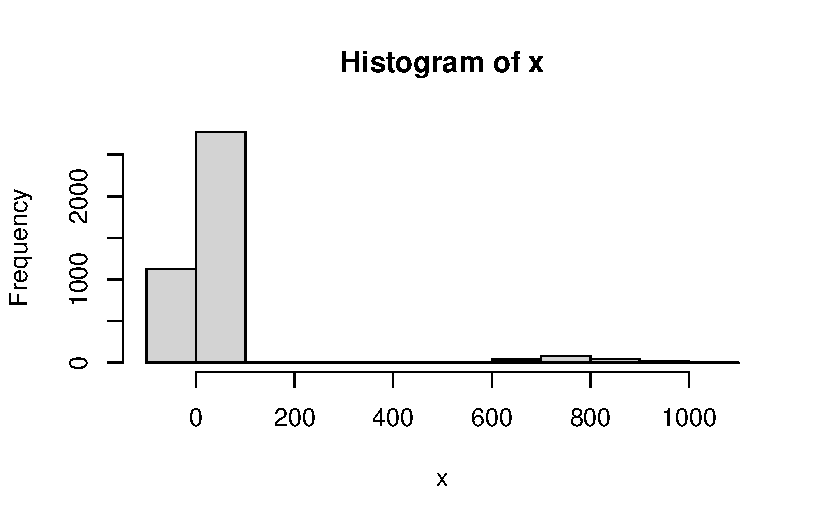
\includegraphics{Homework-1_files/figure-pdf/unnamed-chunk-10-1.pdf}

\begin{verbatim}
.Primitive("return")
\end{verbatim}

\subsubsection{Part l (9 points)}\label{part-l-9-points}

Filter the tibble with all 2025 games to only include Utah Tech or
Southern Utah, then crate a tibble or data frame where each row is a
game played by either team that has one column indicating the school,
Utah Tech or Southern Utah, and a second column indicating the number of
points that team played, regardless of whether the team was home or
away. Then use your \texttt{ggbox()} function to create a side-by-side
boxplot of number of points scored in all 2025 games for each team.

Note, this is a little challenging. The most straightforward way to do
this is to use the \texttt{pivot\_longer()} function with
\texttt{cols\ =} the names of the two columns that have the away and the
home teams (the names of these columns should not be in quotes, but they
should be in a vector \texttt{c()}). Try to do this yourself first, but
using AI for some help is fine.

\begin{Shaded}
\begin{Highlighting}[]
\NormalTok{cbbga8 }\OtherTok{=}\NormalTok{ cbbga7 }\SpecialCharTok{|\textgreater{}}
  \FunctionTok{filter}\NormalTok{(home}\SpecialCharTok{==}\StringTok{\textquotesingle{}Utah Tech\textquotesingle{}}\SpecialCharTok{|}
\NormalTok{           home}\SpecialCharTok{==}\StringTok{"Southern Utah"} \SpecialCharTok{|}
\NormalTok{           visitor }\SpecialCharTok{==} \StringTok{"Utah Tech"}\SpecialCharTok{|}
\NormalTok{           visitor }\SpecialCharTok{==} \StringTok{"Southern Utah"}\NormalTok{)}

\NormalTok{points\_df }\OtherTok{\textless{}{-}}\NormalTok{ cbbga8 }\SpecialCharTok{|\textgreater{}}
  \FunctionTok{select}\NormalTok{(home, visitor, home\_score, visitor\_score) }\SpecialCharTok{|\textgreater{}}
  \FunctionTok{pivot\_longer}\NormalTok{(}
    \AttributeTok{cols =} \FunctionTok{c}\NormalTok{(home, visitor),}
    \AttributeTok{names\_to =} \StringTok{"side"}\NormalTok{,}
    \AttributeTok{values\_to =} \StringTok{"school"}
\NormalTok{  ) }\SpecialCharTok{|\textgreater{}}
  \FunctionTok{mutate}\NormalTok{(}
    \AttributeTok{points =} \FunctionTok{ifelse}\NormalTok{(side }\SpecialCharTok{==} \StringTok{"home"}\NormalTok{, home\_score, visitor\_score)}
\NormalTok{  ) }\SpecialCharTok{|\textgreater{}}
  \FunctionTok{filter}\NormalTok{(school }\SpecialCharTok{\%in\%} \FunctionTok{c}\NormalTok{(}\StringTok{"Utah Tech"}\NormalTok{, }\StringTok{"Southern Utah"}\NormalTok{)) }\SpecialCharTok{|\textgreater{}}
  \FunctionTok{select}\NormalTok{(school, points)}

\FunctionTok{ggbox}\NormalTok{(points\_df, school, }\FunctionTok{as.numeric}\NormalTok{(points))}
\end{Highlighting}
\end{Shaded}

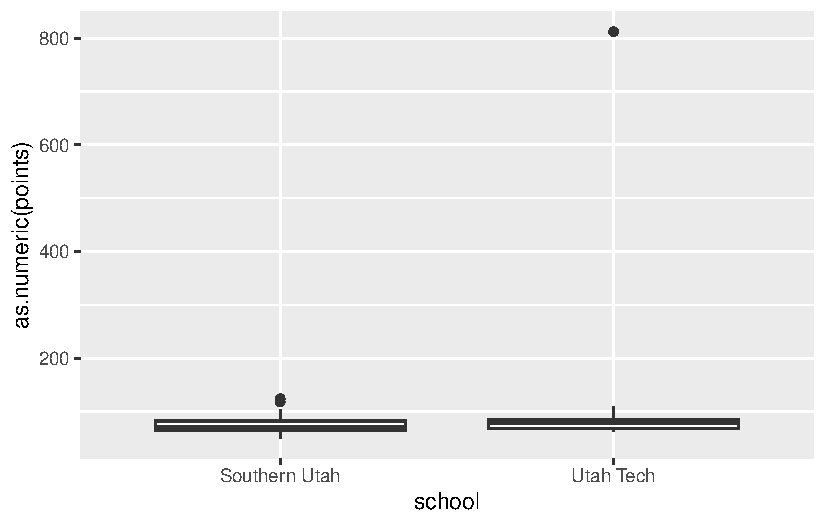
\includegraphics{Homework-1_files/figure-pdf/unnamed-chunk-11-1.pdf}

\subsubsection{Part m (5 points)}\label{part-m-5-points}

Create one more appropriate graphs for the 2025 basketball data. This
graph could be anything you'd like as long as you use \texttt{ggplot2},
it shows something meaningful, and it is not the same as the graphs you
made in parts k or l.

\begin{Shaded}
\begin{Highlighting}[]
\FunctionTok{ggplot}\NormalTok{(points\_df, }\FunctionTok{aes}\NormalTok{(}\AttributeTok{x=}\NormalTok{school, }\AttributeTok{y=}\NormalTok{points)) }\SpecialCharTok{+}
  \FunctionTok{geom\_bar}\NormalTok{(}\AttributeTok{stat=}\StringTok{"identity"}\NormalTok{)}
\end{Highlighting}
\end{Shaded}

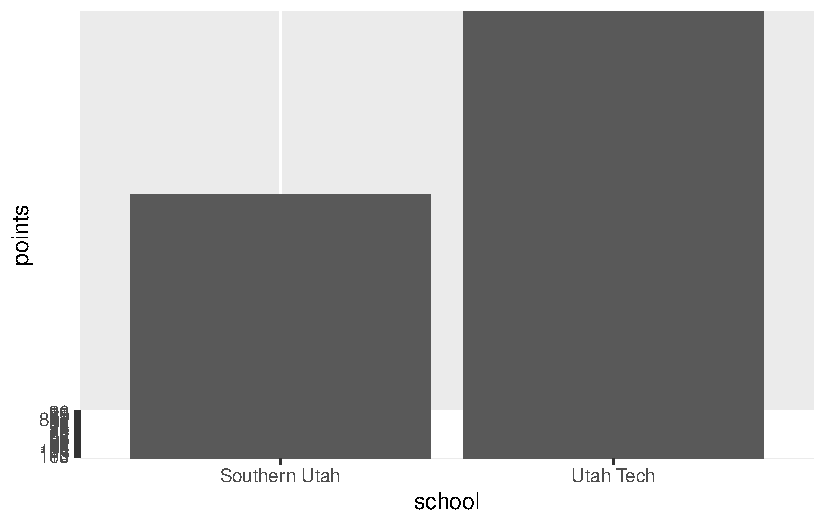
\includegraphics{Homework-1_files/figure-pdf/unnamed-chunk-12-1.pdf}

\section{Problem 3 (15 points)}\label{problem-3-15-points}

Repeat parts b-e and g of Problem 2 using Python in Quarto. First, pass
the original object that you read in from the website to Python without
any changes to it (you do not need to read the file from the web in
Python, but you can if you'd like) and then use \texttt{pandas} (or
\texttt{polars} if you'd like) to rename the columns as indicated in
part b, add the columns specified in part c, arrange the data as in part
d, drop the ``garbage'' column as in part e, and filter it down as in
part g. The \texttt{pandas} functions \texttt{rename}, \texttt{assign}
(instead of \texttt{mutate}), \texttt{drop} (instead of \texttt{select})
and \texttt{str.contains} (used to select the right rows) will be useful
here. Be sure to follow the guide in Notes 3 to properly install Python,
install the \texttt{pandas} library and to load it in \textbf{R}.




\end{document}
